\noindent
This chapter describes the type of data that is required to run a forward problem with OpenMEEG.
More detail on the data format is provided in Appendix~\ref{chap:format}.

\noindent
\underline{Meshes}~:\\
Meshes describing the interfaces between regions of homogeneous conductivity. These meshes generally represent:
\begin{itemize}
    \item the inner skull surface
    \item the outer skull surface
    \item the outer scalp surface
\end{itemize}

\noindent
The recommended mesh size is approximately 600 to 800 points per surface.


\medskip

\centerline{
    \hbox{\parbox[t]{5.5cm}{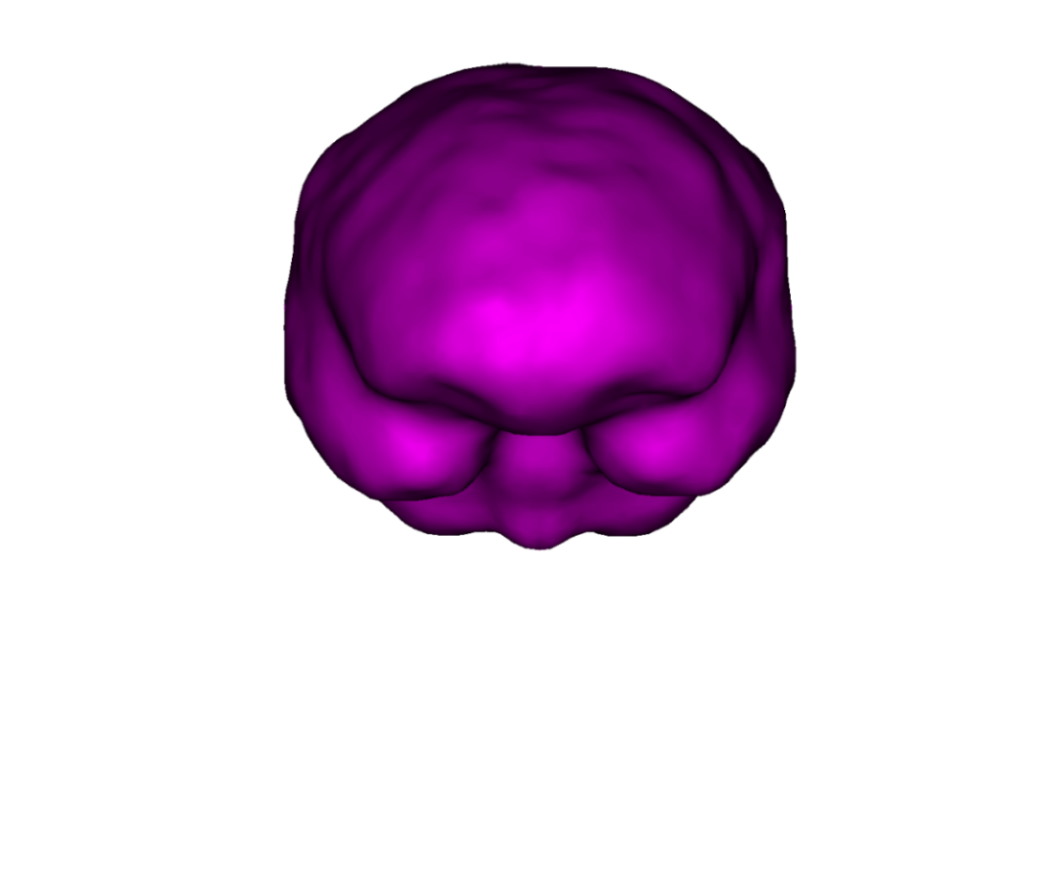
\includegraphics[width=5cm]{tete_couches_brain.png}\\
                            \parbox{5cm}{External surface of the cortex}}
          \parbox[t]{5.5cm}{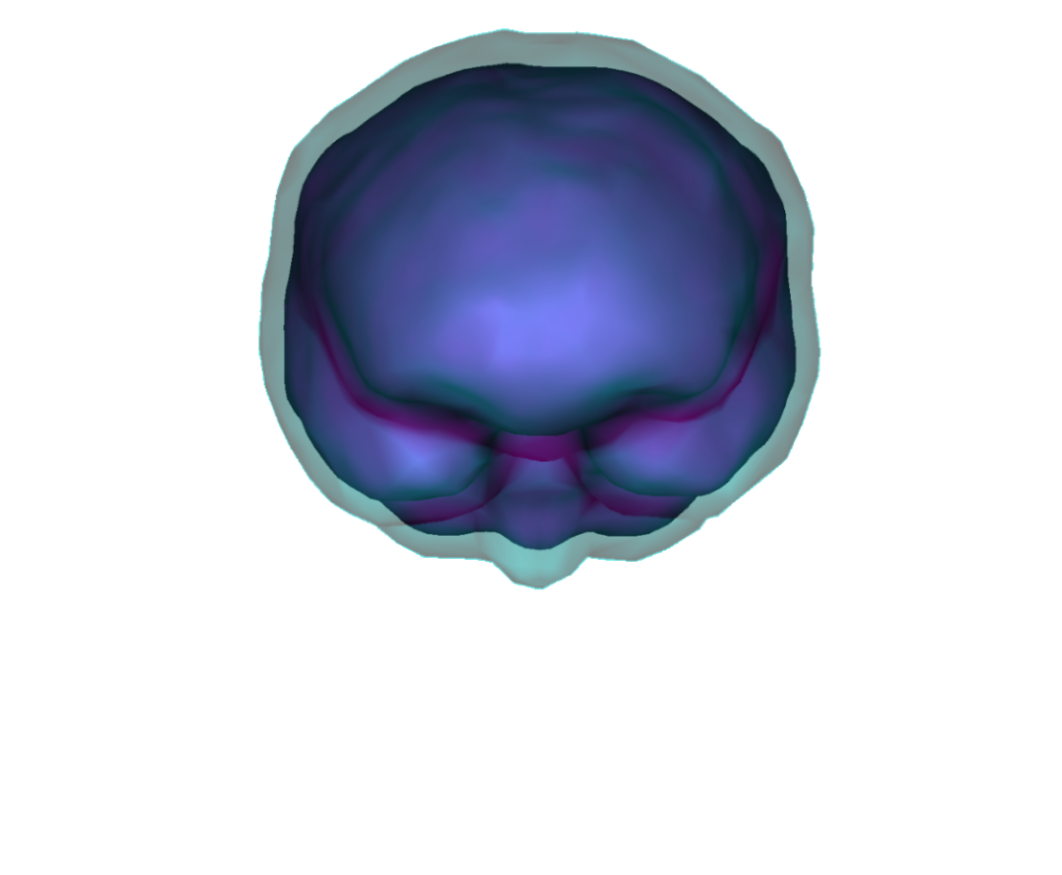
\includegraphics[width=5cm]{tete_couches_brainskull.png}\\\parbox{5cm}{External surface of the skull in blue and external surface of the cortex in fuchsia}}
          \parbox[t]{5.5cm}{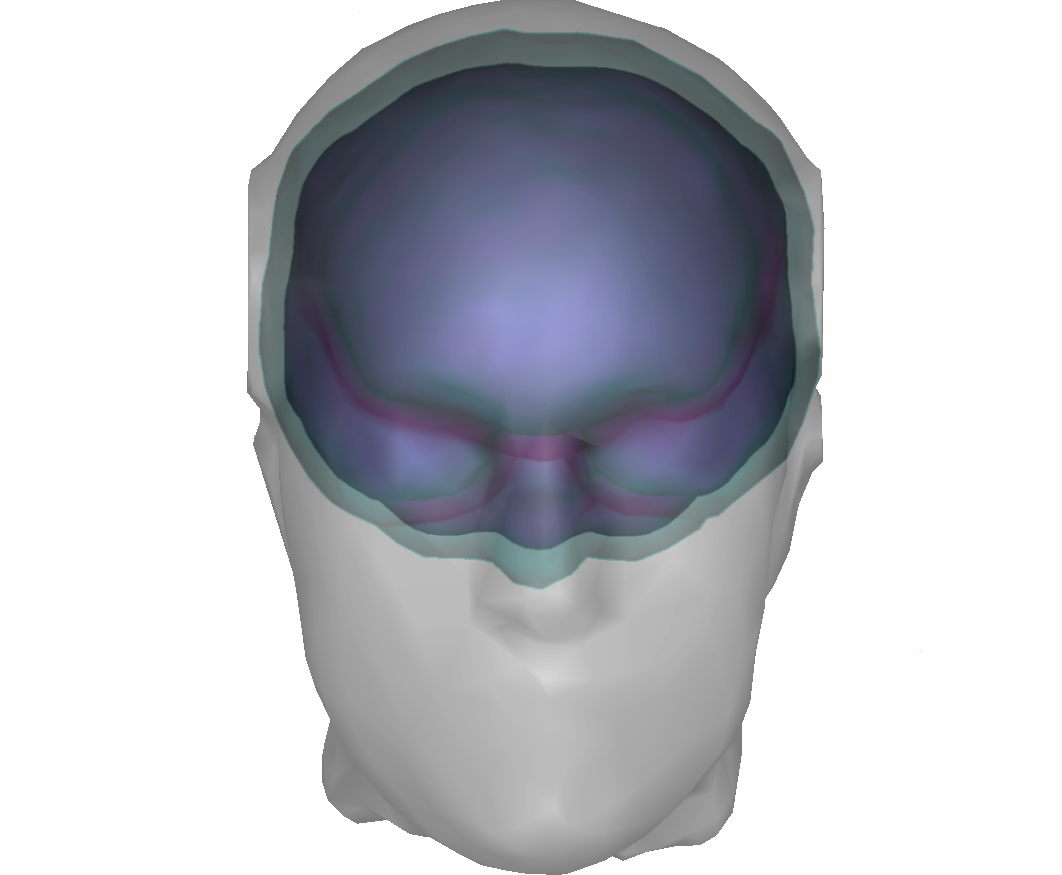
\includegraphics[width=5cm]{tete_couches_brainskullhead.png}\\
                            \parbox{5cm}{Example with three surfaces~:
                                  \begin{itemize}
                                       \item outer scalp (gray)
                                       \item outer skull (blue)
                                       \item inner skull (pink)
                                  \end{itemize}}
                            }
    }
}

\bigskip
\noindent
\underline{Sources}~:\\
Sources can be of two types: isolated or distributed. 
\noindent
For distributed sources, a source mesh describes their support. This is a detailed mesh generally covering the whole cortex. The mesh size should not exceed 35 000 points. 
The source amplitude is represented as continuous, and linear on each of the mesh triangles. The source orientation is modeled
as piecewise constant, normal to each of the mesh triangles.
\begin{center}
    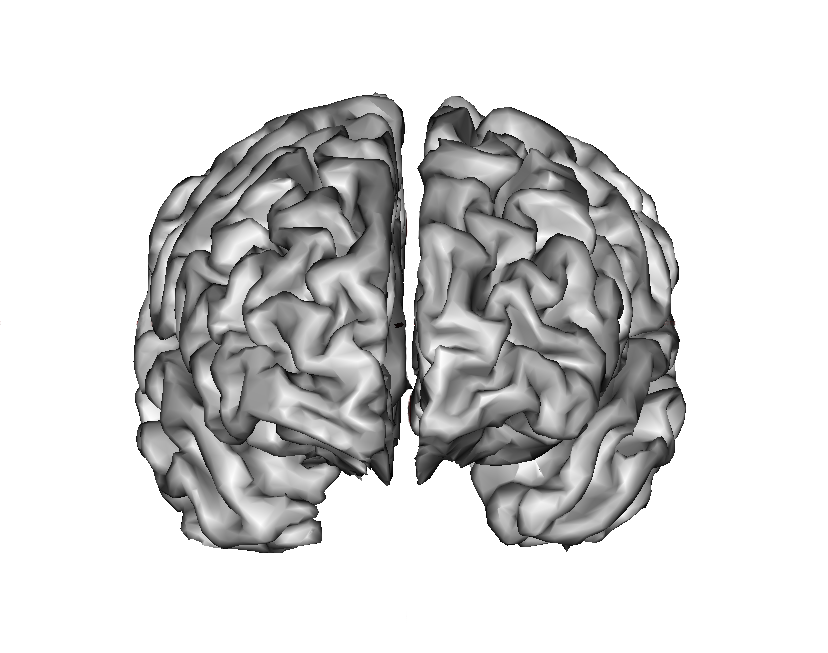
\includegraphics[height=9cm]{cortex.png}\\
Source mesh
\end{center}
\noindent
Isolated sources are the superposition of current dipoles, each of which is defined by its position and its moment.

\noindent
\underline{Sensors}~:
For EEG, the sensors are defined by the list of the x-y-z coordinates of the electrode positions. The electrodes are considered punctual and are called {\em patches}.	
The MEG sensor description is more complex, see  Appendix~\ref{chap:format}.
